\section{Theme computation}
\label{sec:theme computation}

To identify the tactical themes present in a generated position, we employ the Lichess puzzler pipeline \cite{lichesspuzzler}, which iterates over the principal variation to detect specific themes. We group these themes into several distinct categories, which include the following: state of game, type of endgame, type of checkmate, length of checkmate, length of puzzle, winning states, and other tactics. Table \ref{tab:themes} enumerates every specific theme we evaluate during the puzzle evaluation process. While the Lichess puzzles dataset \cite{lichesspuzzledatabase} contains additional metadata tags, we exclusively focus on objective, position-based themes. We intentionally discard the other tags, such as ``master vs. master'', as they cannot be verified from the board state alone.

During reinforcement learning and evaluation, we determine whether a generated puzzle successfully matches the requested conditions by comparing the generated theme set $\mathcal{T}_{\text{gen}}$ against the requested theme set $\mathcal{T}_{\text{req}}$. Rather than requiring a strict superset match $\mathcal{T}_{\text{req}} \subseteq \mathcal{T}_{\text{gen}}$, we use the specific groups for the check. The complete theme matching logic is detailed in Algorithm \ref{alg:theme match}.

\begin{table}[h]
    \centering
    \renewcommand{\arraystretch}{1.3}
    \begin{tabular}{l p{10cm}}
        \hline
        \textbf{Category} & \textbf{Themes} \\
        \hline
        State-of-game & Opening, Middlegame, Endgame \\
        Type-of-endgame & Pawn endgame, Bishop endgame, Knight endgame, Rook endgame, Queen endgame, Queen rook endgame \\
        Type-of-checkmate & Mate, Back rank mate, Boden mate, Smothered mate, Hook mate, Double bishop mate, Arabian mate, Dovetail mate, Anastasia mate \\
        Length-of-checkmate & Mate in 1, Mate in 2, Mate in 3, Mate in 4, Mate in 5 \\
        Length-of-puzzle & One move, Short, Long, Very long \\
        Winning & Crushing, Advantage \\
        Other & Hanging piece, Fork, Interference, Kingside attack, Zugzwang, Exposed king, Skewer, Pin, Quiet move, Discovered attack, Sacrifice, Deflection, Advanced pawn, Attraction, Promotion, Queenside attack, Defensive move, Attacking f2/f7, Clearance, Intermezzo, Equality, Trapped piece, X-ray attack, Capturing defender, Double check, En passant, Castling, Underpromotion \\
        \hline
    \end{tabular}
    \caption{The complete list of themes supported by the Lichess puzzler pipeline, grouped by their respective categories.}
    \label{tab:themes}
\end{table}

\begin{algorithm}[H]
    \caption{Themes match}
    \label{alg:theme match}
    \begin{algorithmic}
        \Require Requested themes $\mathcal{T}_{\text{req}}$, Generated puzzle themes $\mathcal{T}_{\text{gen}}$
        \Require Category sets $\mathcal{S}_{\text{state}}$, $\mathcal{S}_{\text{endgame}}$, $\mathcal{S}_{\text{mate\_len}}$, $\mathcal{S}_{\text{mate\_type}}$, $\mathcal{S}_{\text{other}}$
        
        \If{$(\mathcal{T}_{\text{req}} \cap \mathcal{S}_{\text{state}}) \not\subseteq \mathcal{T}_{\text{gen}}$}
            \State \textbf{return} False
        \EndIf
        
        \If{\text{``endgame''} $\in \mathcal{T}_{\text{req}}$}
            \If{$(\mathcal{T}_{\text{req}} \cap \mathcal{S}_{\text{endgame}}) \not\subseteq \mathcal{T}_{\text{gen}}$}
                \State \textbf{return} False
            \EndIf
        \EndIf
        
        \If{\text{``mate''} $\in \mathcal{T}_{\text{req}}$}
            \If{\text{``mate''} $\notin \mathcal{T}_{\text{gen}}$}
                \State \textbf{return} False
            \EndIf
            \If{$(\mathcal{T}_{\text{req}} \cap \mathcal{S}_{\text{mate\_len}}) \not\subseteq \mathcal{T}_{\text{gen}}$}
                \State \textbf{return} False
            \EndIf
            \If{$(\mathcal{T}_{\text{req}} \cap \mathcal{S}_{\text{mate\_type}}) \not\subseteq \mathcal{T}_{\text{gen}}$}
                \State \textbf{return} False
            \EndIf
        \Else
            \If{$(\mathcal{T}_{\text{req}} \cap \mathcal{S}_{\text{other}}) \not\subseteq \mathcal{T}_{\text{gen}}$}
                \State \textbf{return} False
            \EndIf
        \EndIf
        
        \State \textbf{return} True
    \end{algorithmic}
\end{algorithm}




\section{Supervised training}


In addition to the training metrics presented in Figure \ref{fig:supervised_training_metrics}, we also monitor the model's performance during supervised training by evaluating generated samples conditioned on themes drawn from the held-out test set. These test-set evaluation metrics are illustrated in Figure \ref{fig:supervised_training_test_metrics}. We observe that while the legal rate and uniqueness rate saturate after approximately 1,000,000 training steps, the counter-intuitiveness and overall puzzle rates converge significantly faster. However, the inherent variance in the counter-intuitiveness metric makes identifying the precise convergence point of the puzzle rate challenging. We observe that the performance of these metrics do not decrease similarly to the test loss in Figure \ref{fig:training_loss}. We still select the checkpoint at 1,000,000 training steps, as the metrics do not improve with more training.

\begin{figure}[h]
    \centering
    
\includegraphics[width=0.49\linewidth]{sections/figures/supervised_training_progress/test/Legal_rate.pdf}
    \hfill
    
\includegraphics[width=0.49\linewidth]{sections/figures/supervised_training_progress/test/Uniqueness_rate.pdf}
    
    \vspace{0.5cm}
    
    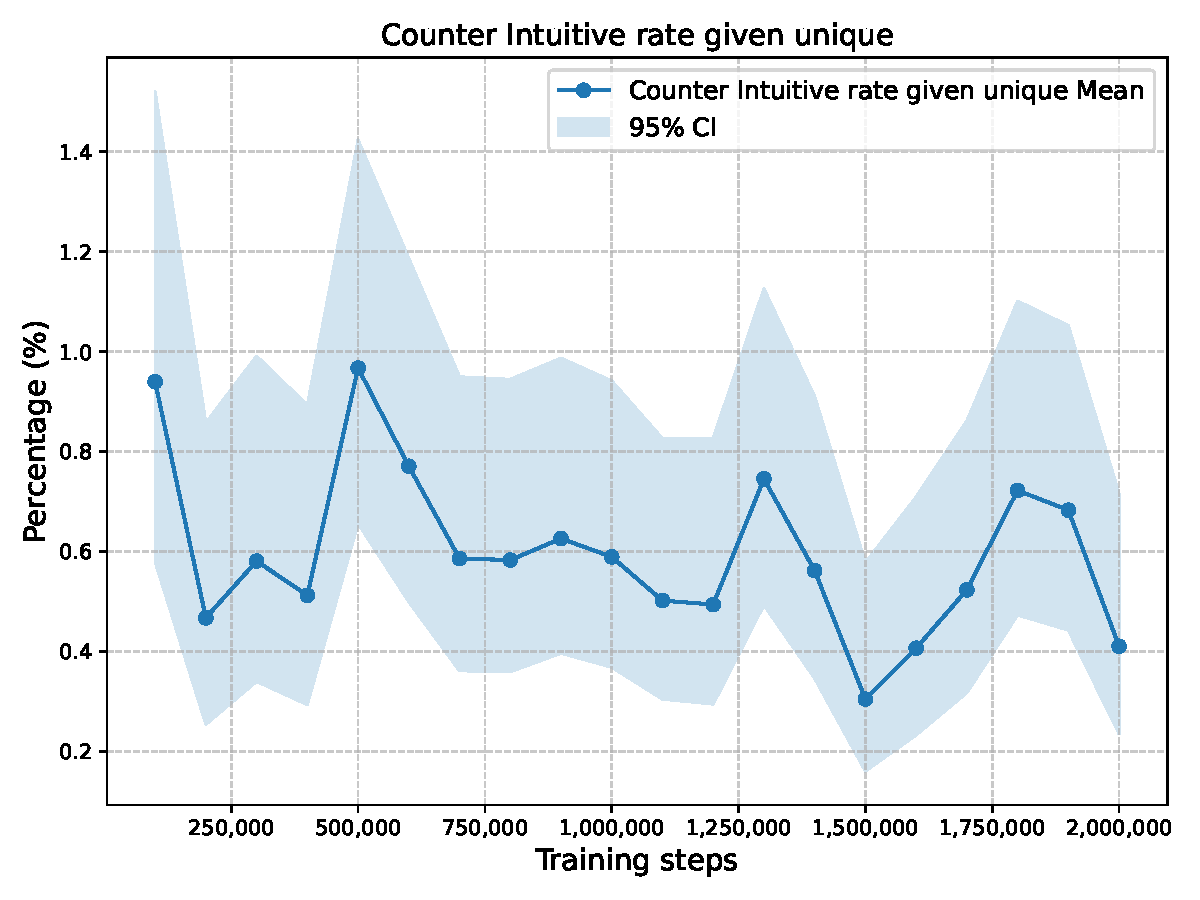
\includegraphics[width=0.49\linewidth]{sections/figures/supervised_training_progress/test/Counter_intuitive_rate_given_unique.pdf}
    \hfill
    
\includegraphics[width=0.49\linewidth]{sections/figures/supervised_training_progress/test/Puzzle_rate.pdf}
    \caption{Evolution of the primary quality metrics with context from the testing set during supervised pretraining.}
    \label{fig:supervised_training_test_metrics}
\end{figure}


To further benchmark our the performance of our model, we additionally sample from the model with a lower temperature of 0.1 \ref{tab:supervised metrics low temperature}. We notice that with the almost greedy sampling, the uniqueness is considerably improved, whereas, the counter-intuitiveness is not. Furthermore, the difference between the move sampling is further amplified, as if we sample the move after sampling the position, the uniqueness is considerably lower than if the move was sampled simultaneously to the position. We conclude that the best move prediction improves the model performance meaningfully. This improvement comes at a cost to the distance metrics though, as the board distance to the Lichess dataset is around 6.91 and the PV distance is 0.80 when sampling with a low temperature.

\begin{table}[h]
    \centering
    \caption{The final metrics after supervised training with different context distributions. The sampling is performed with a temperature $0.1$ and $256$ denoising steps.}
    \resizebox{\textwidth}{!}{
    \begin{tabular}{|c|c|c|c|c|c|c|}
        \hline
        Context & Sampling & Legal & Unique & Counter-intuitive | unique & Puzzle & Theme\\
        \hline\hline
        Train & block & 98.04 $\pm$ 0.27 & 35.20 $\pm$ 0.93 & 0.50 $\pm$ 0.081 & 0.18 $\pm$ 0.081 & 90.18 $\pm$ 0.90 \\
        Train & normal & 99.44 $\pm$ 0.14 & 42.01 $\pm$ 0.96 & 0.63 $\pm$ 0.099 & 0.26 $\pm$ 0.099 & 92.75 $\pm$ 0.94 \\
        Test & block & 98.33 $\pm$ 0.25 & 34.89 $\pm$ 0.92 & 0.50 $\pm$ 0.081 & 0.18 $\pm$ 0.081 & 89.98 $\pm$ 0.90 \\
        Test & normal & 99.45 $\pm$ 0.14 & 42.37 $\pm$ 0.96 & 0.48 $\pm$ 0.088 & 0.21 $\pm$ 0.088 & 92.90 $\pm$ 0.95 \\
        \hline\hline
        \multicolumn{2}{|c|}{Lichess puzzles} & \textbf{100.0} $\pm$ 0.0 & \textbf{83.58} $\pm$ 0.23 & \textbf{1.55} $\pm$ 0.070 & \textbf{1.29} $\pm$ 0.070 & \textbf{100.0} $\pm$ 0.0\\
        \hline
    \end{tabular}
    }
    \label{tab:supervised metrics low temperature}
\end{table}


\section{Reinforcement learning}
\label{sec:RL appendix}

\subsection{Additional results}

In this section, we present a few additional results on the reinforcement learning. We begin our experiments by training a model with using only the legality, uniqueness and counter-intuitiveness as the components of the reward. In Figure \ref{fig:rl_overfit_metrics}, we observe the results of such a training run. We observe that the model collapses after around 1700 training steps. For this run, we use a learning rate of $3\cdot10^{-5}$ with $\mu=2$ gradient updates per batch and 32 groups of 6 generations with the same themes. Compared to the results of \citeauthor{feng2025generatingcreativechesspuzzles}, we see that the masked diffusion model is more resistant to overfitting compared to an LLM and takes a lot longer to collapse. This is supported by the findings of \citeauthor{nie2025scalingmaskeddiffusionmodels}, although our results are for reinforcement learning, whereas their results concern pretraining.

\begin{figure}[h]  % ddpo/Ablations/no_diversity_filtering
    \centering
    \begin{subfigure}[t]{0.48\textwidth}
        \centering
        
\includegraphics[width=\textwidth]{sections/figures/rl_training_progress/overfit/reward.pdf}
        \caption{Reward over training steps.}
        \label{fig:overfit_reward}
    \end{subfigure}
    \hfill
    \begin{subfigure}[t]{0.48\textwidth}
        \centering
        
\includegraphics[width=\textwidth]{sections/figures/rl_training_progress/overfit/unique_and_counter_intuitive.pdf}
        \caption{Puzzle rate over training steps.}
        \label{fig:overfit_unique}
    \end{subfigure}
    \vspace{0.5cm}
    \begin{subfigure}[t]{0.48\textwidth}
        \centering
        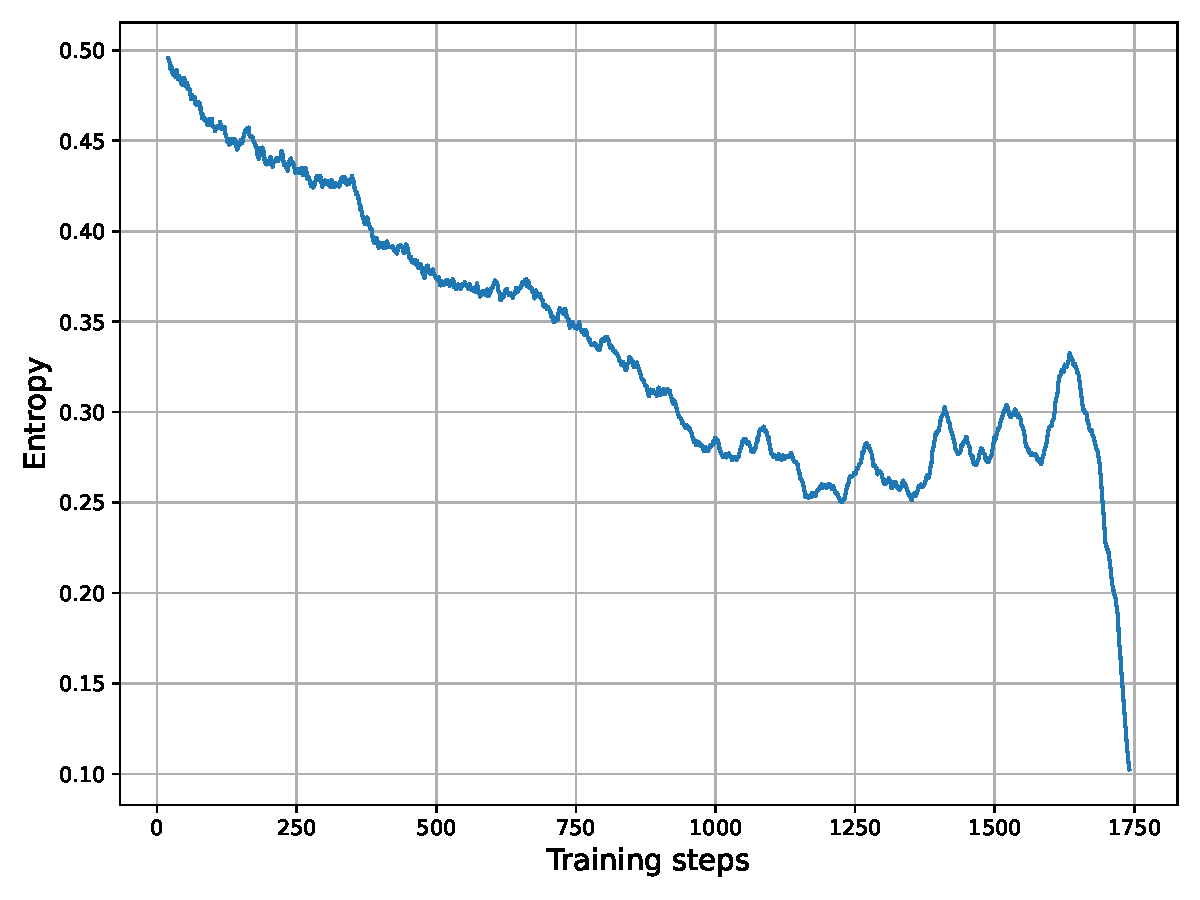
\includegraphics[width=\textwidth]{sections/figures/rl_training_progress/overfit/entropy.pdf}
        \caption{Entropy over training steps.}
        \label{fig:overfit_entropy}
    \end{subfigure}
    \hfill
    \begin{subfigure}[t]{0.48\textwidth}
        \centering
        
\includegraphics[width=\textwidth]{sections/figures/rl_training_progress/overfit/kl_divergence.pdf}
        \caption{KL divergence over training steps.}
        \label{fig:overfit_kl}
    \end{subfigure}
    \caption{An illustration of DDPO training with just legality, uniqueness and counter-intuitiveness based reward. We observe model collapse at around 1700 training steps.}
    \label{fig:rl_overfit_metrics}
\end{figure}

To combat model collapse, we introduce many diversity filtering mechanisms inspired by \cite{feng2025generatingcreativechesspuzzles}. We introduce the methods described in section \ref{sec:reward function} and perform manual hyperparameter search for a good value of the entropy coefficient $\gamma$. In Figure \ref{fig:entropy coef search} we observe that with a high entropy bonus coefficient $\gamma = 0.3$, the task is too difficult for our model to learn, but with a lower entropy bonus coefficient $\gamma = 0.03$ or $\gamma = 0.06$, the entropy slowly decreases.

\begin{figure}[h]  % ddpo/Ablations/all_diversity_filtering_kl_entropy_with_grad, ddpo/Ablations/all_diversity_filtering_kl_entropy_with_grad_large_entropy_coef, ddpo/Ablations/all_diversity_filtering_kl_entropy_with_grad_medium_entropy_coef
    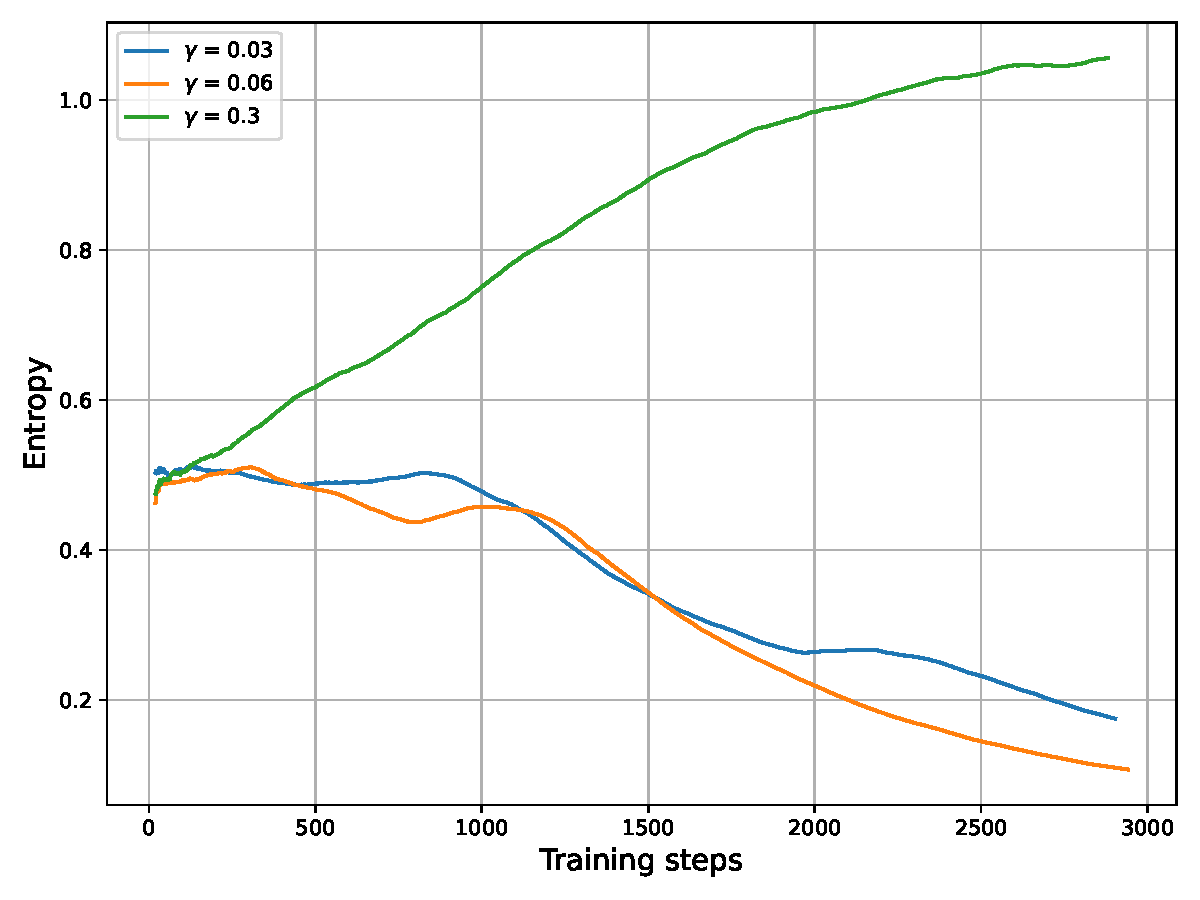
\includegraphics[width=0.49\textwidth]{sections/figures/rl_training_progress/overfit/DDPO/entropies.pdf}
    \hfill
    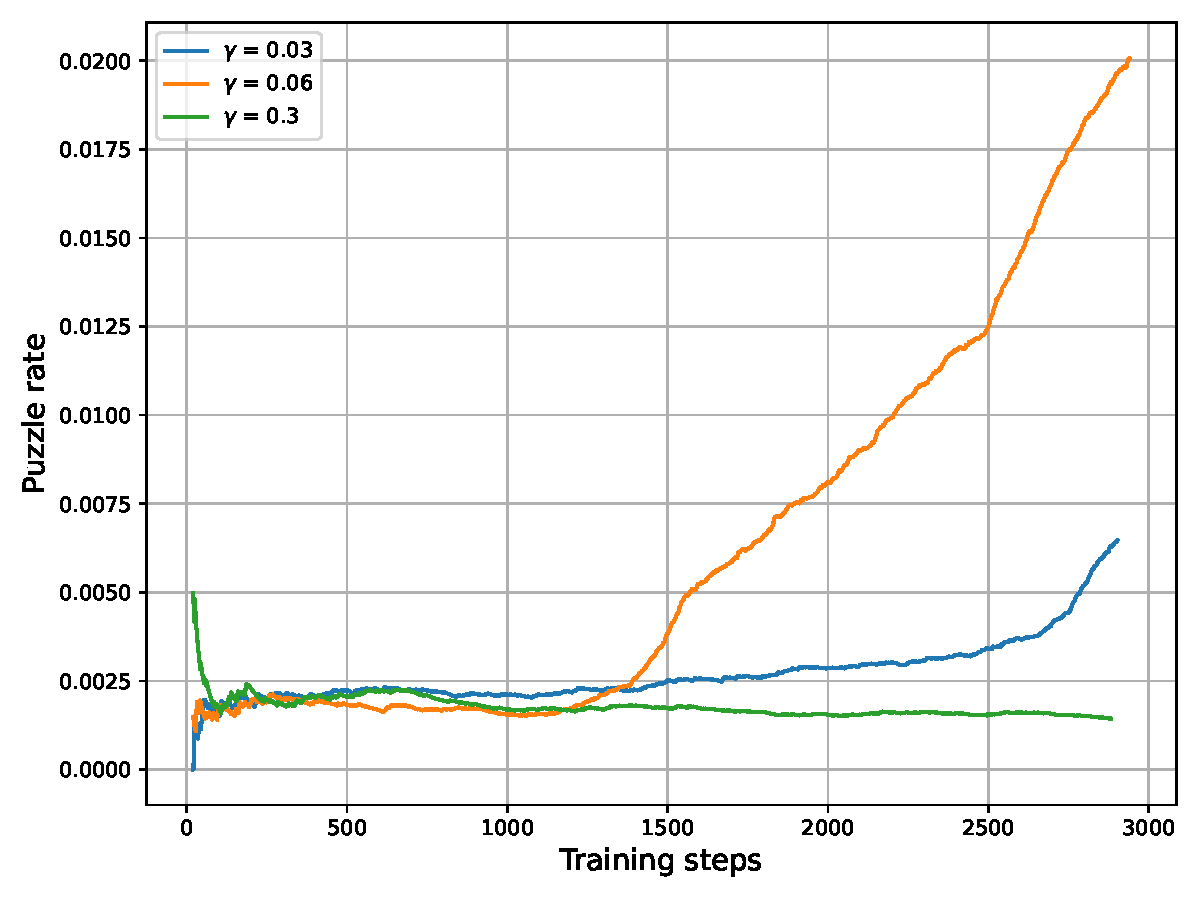
\includegraphics[width=0.49\textwidth]{sections/figures/rl_training_progress/overfit/DDPO/uniques_and_counter_intuitives.pdf}
    \caption{The training progress with different values of $\gamma$. We observe, that the two lower values overfit, whereas, the larger one does not learn.}
    \label{fig:entropy coef search}
\end{figure}


In Figures \ref{fig:theme_dist}, we present the distributions of themes in the lichess dataset as well as the generated positions. In Figure \ref{fig:ci_over_themes}, we present the counter-intuitive rates for each of these themes. We notice that it is considerably more difficult to generate counter-intuitive positions. For instance, although mate-in-one puzzles are quite common, no counter-intuitive mate-in-ones are present in the Lichess dataset or the generated positions.


\begin{figure}[h]
    \centering
    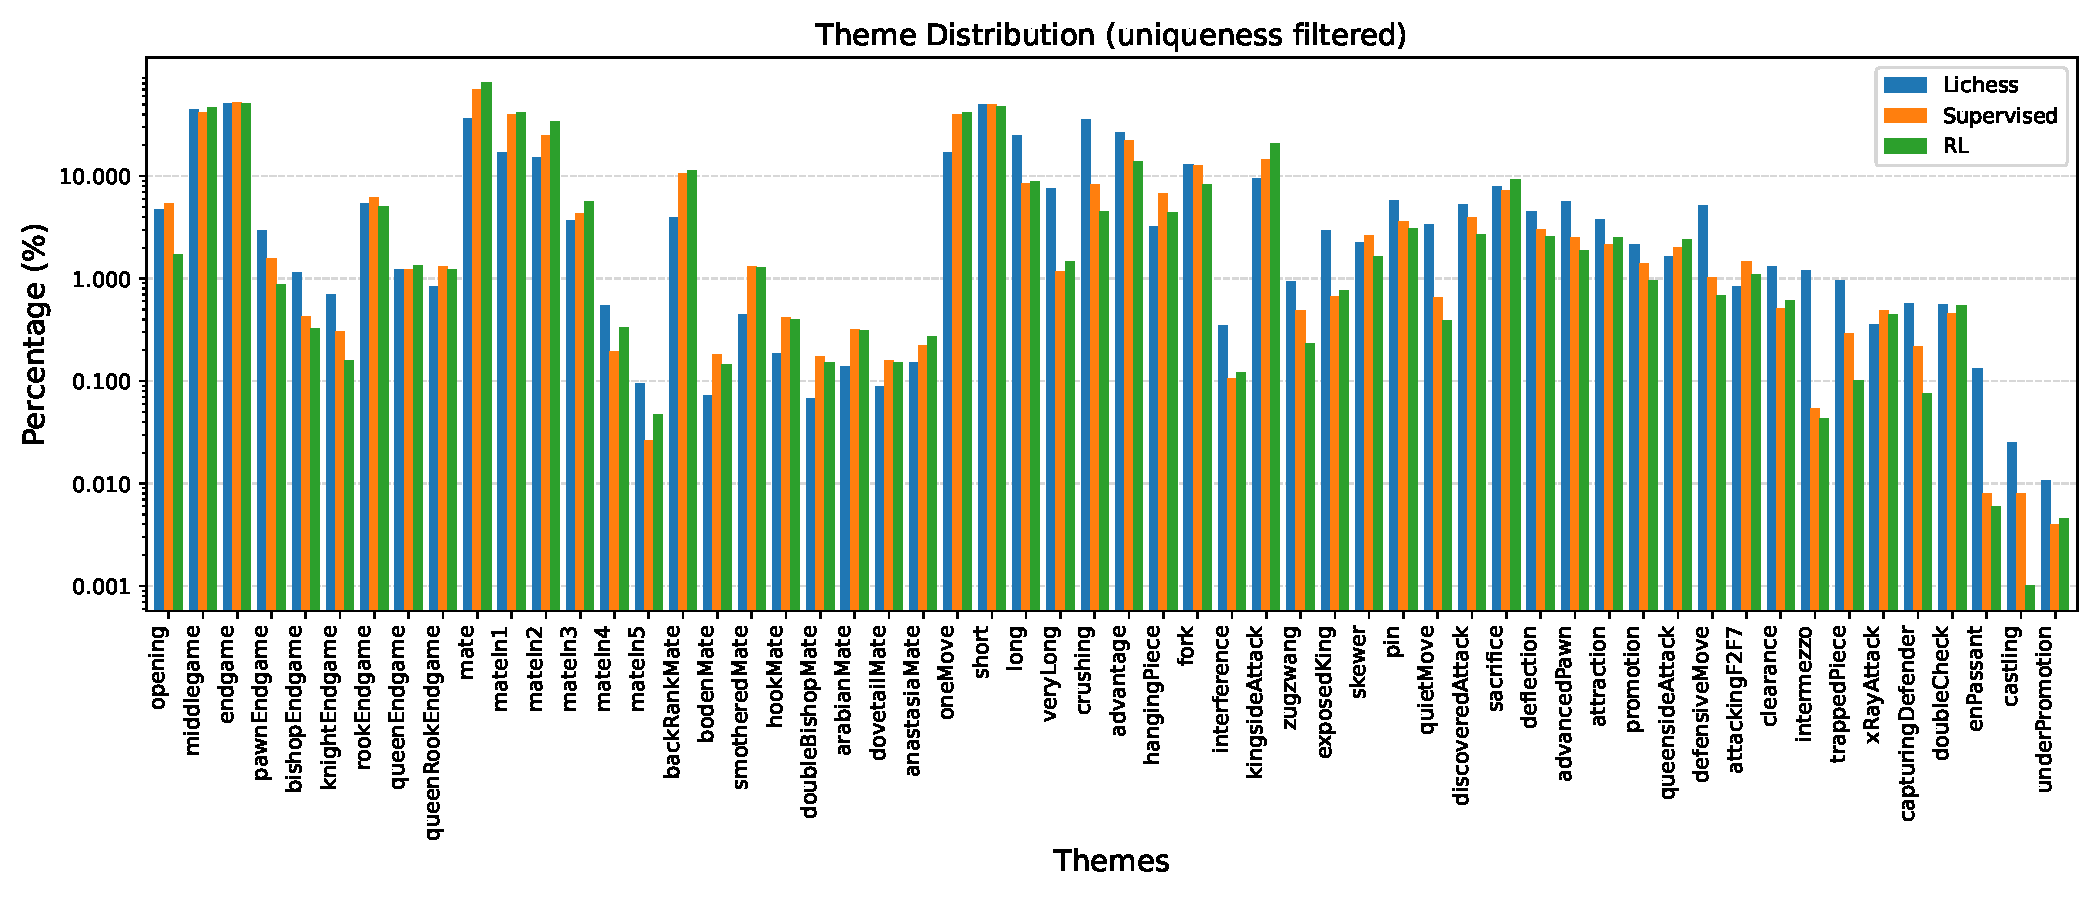
\includegraphics[width=\textwidth]{sections/figures/other/theme_distribution.pdf}
    \caption{The distribution of themes for the Lichess puzzles dataset, our supervised model and the final model. All positions are first filtered for positions with a unique solutions and the percentages are computed accross the filtered dataset.}
    \label{fig:theme_dist}
\end{figure}

\begin{figure}[h]
    \centering
    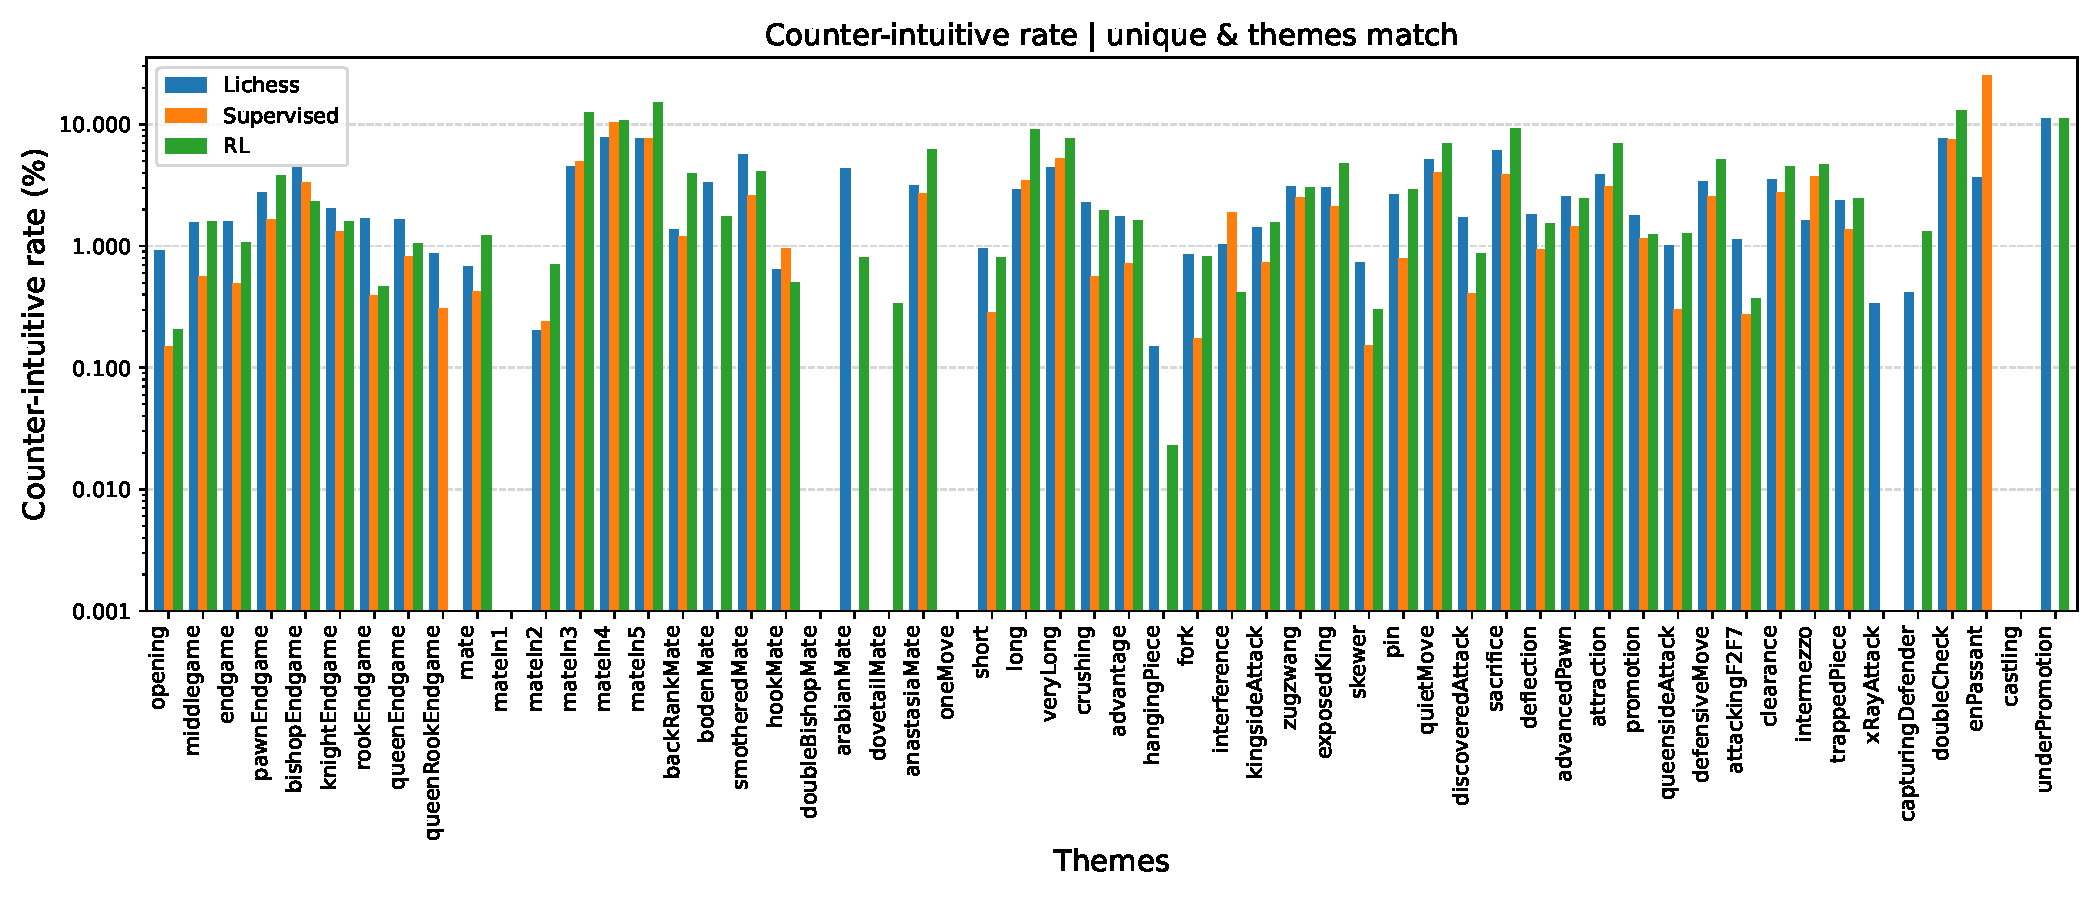
\includegraphics[width=\textwidth]{sections/figures/other/ci_distribution_over_themes.pdf}
    \caption{The counter-intuitive rate for the Lichess puzzles dataset, our supervised model and the final model accross all themes. All positions are first filtered for positions with a unique solutions and so that the themes match the ones the model was conditioned on and the percentages are computed accross the filtered dataset.}
    \label{fig:ci_over_themes}
\end{figure}



\subsection{ELBO-based Sequence-level Policy Optimization}

Before deciding to use DDPO, we attempt to use the ELBO-based sequence-level policy optimization (ESPO) algorithm \cite{ou2025principledrldiffusionllms}. ESPO is an algorithm specifically designed for masked diffusion language models, which led us to consider it first. Although we found some promising results, we were unable to get the model to learn effectively. In Figure \ref{fig:rl_overfit_metrics_ESPO}, we see that we are able to make the model find a puzzle, which produces high rewards, however, after introducing diversity filtering and other reward components, the model either marginally improved without meaningful progress or collapsed to illegal positions depending on the exact configuration. Interestingly, in Figure \ref{fig:rl_overfit_metrics_ESPO}, the model collapse happens quite a lot faster than for DDPO in Figure \ref{fig:rl_overfit_metrics} despite us using a lower learning rate $3\cdot10^{-6}$ with $\mu = 8$. We suspect the faster collapse could be related to ESPO making more efficient updates due to the sequence-level nature of the algorithm.

\begin{figure}[h]  % test/run6
    \begin{subfigure}[t]{0.48\textwidth}
        \centering
        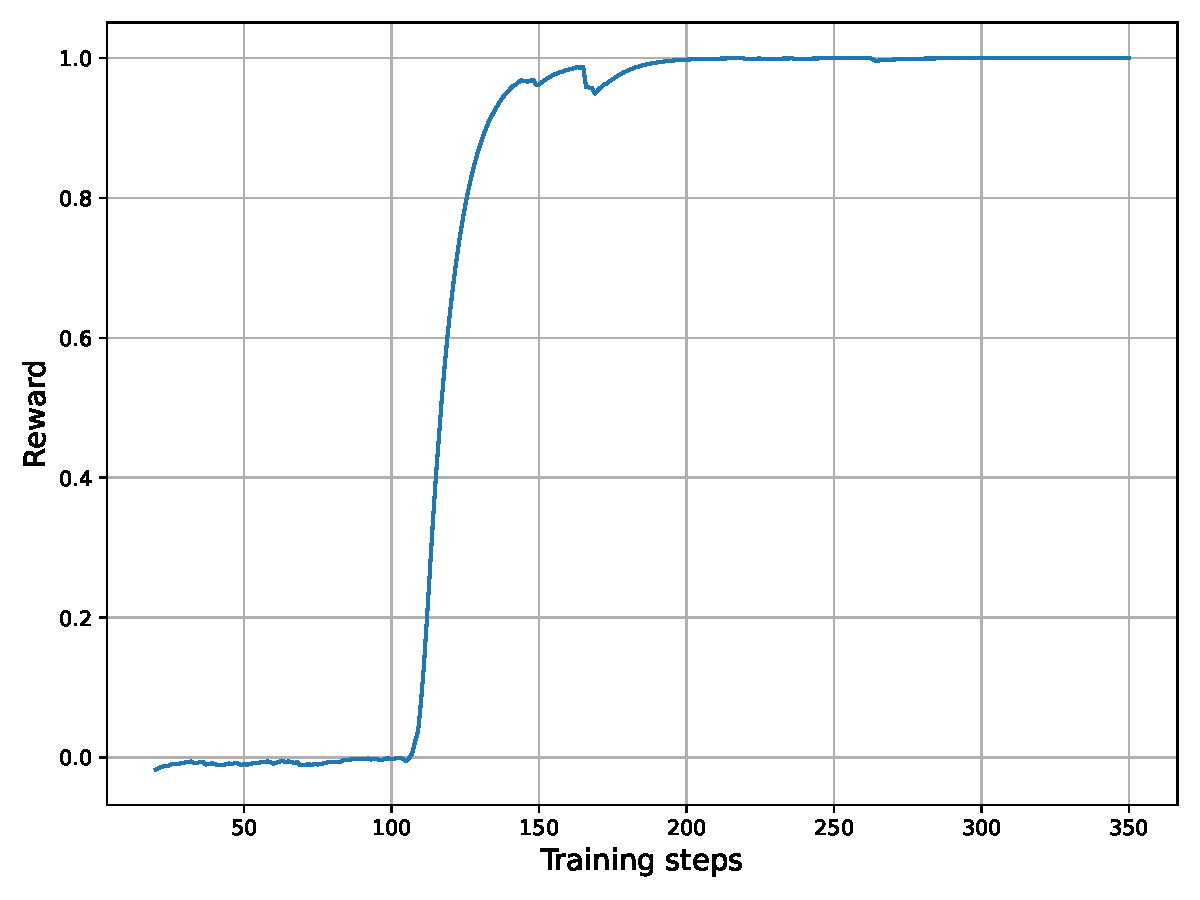
\includegraphics[width=\textwidth]{sections/figures/rl_training_progress/overfit/ESPO/reward.pdf}
        \caption{Reward over training steps.}
        \label{fig:overfit_entropy_ESPO}
    \end{subfigure}
    \hfill
    \begin{subfigure}[t]{0.48\textwidth}
        \centering
        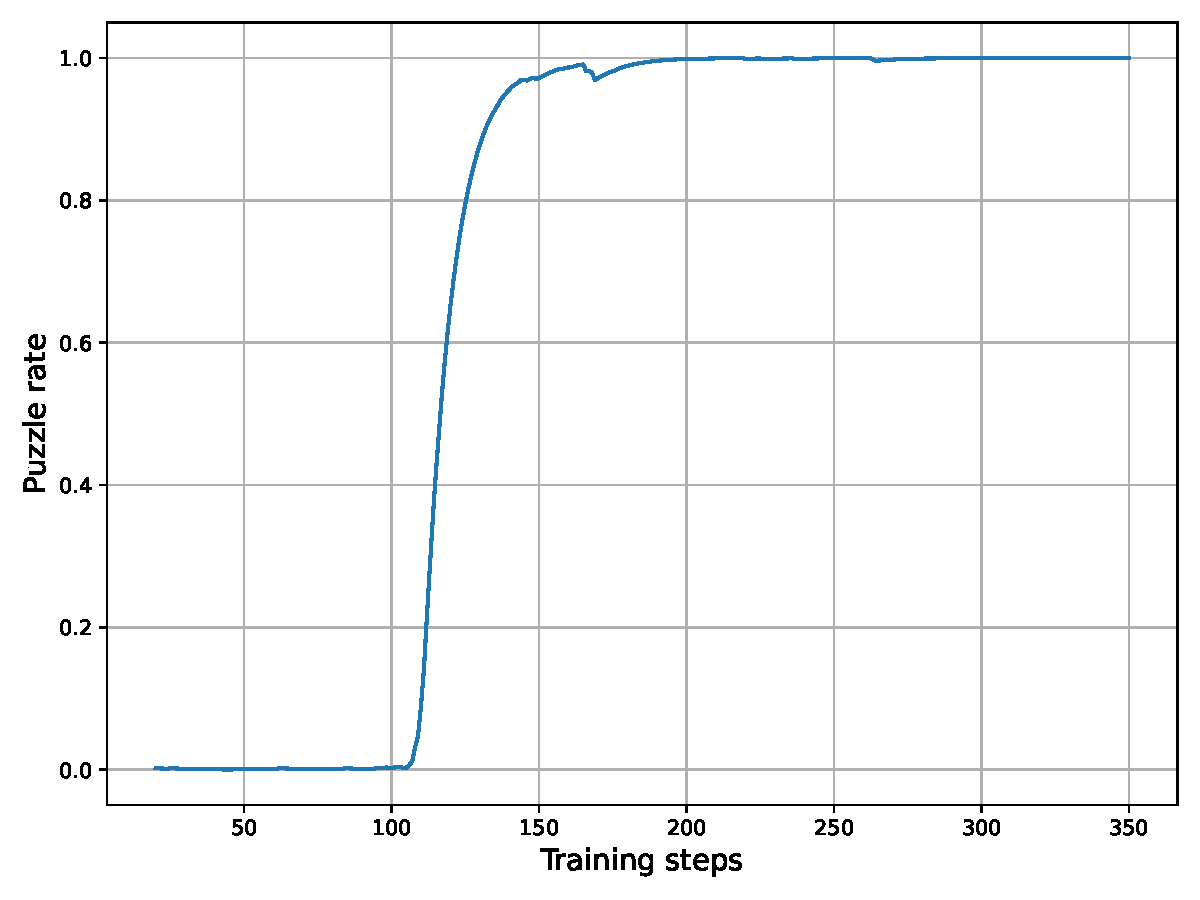
\includegraphics[width=\textwidth]{sections/figures/rl_training_progress/overfit/ESPO/unique_and_counter_intuitive.pdf}
        \caption{Puzzle rate over training steps.}
        \label{fig:overfit_kl_ESPO}
    \end{subfigure}
    \caption{An illustration of ESPO training with just legality, uniqueness and counter-intuitiveness based reward. We observe model collapse at around 110 training steps.}
    \label{fig:rl_overfit_metrics_ESPO}
\end{figure}

After observing model collapse, we enable all diversity filtering mechanisms described in section \ref{sec:reward function}. In figure \ref{fig:espo collapse}, we observe that the model collapses to generate illegal positions. Although, the model improved in figure \ref{fig:rl_overfit_metrics_ESPO}, we observe no meaningful improvement in figure \ref{fig:espo collapse} even in the beginning of the training despite using the same training algorithm. At around 400 training steps, we observe huge gradient spikes and despite using gradient norm clipping, the model collapses to generate completely empty boards with no pieces. In addition to this run, we experimented with ESPO a lot, but were unable to get meaningful improvement to the model without complete mode collapse.

\begin{figure}  % final_thesis_experiments/overfit3_espo and final_thesis_experiments/overfit4_espo
    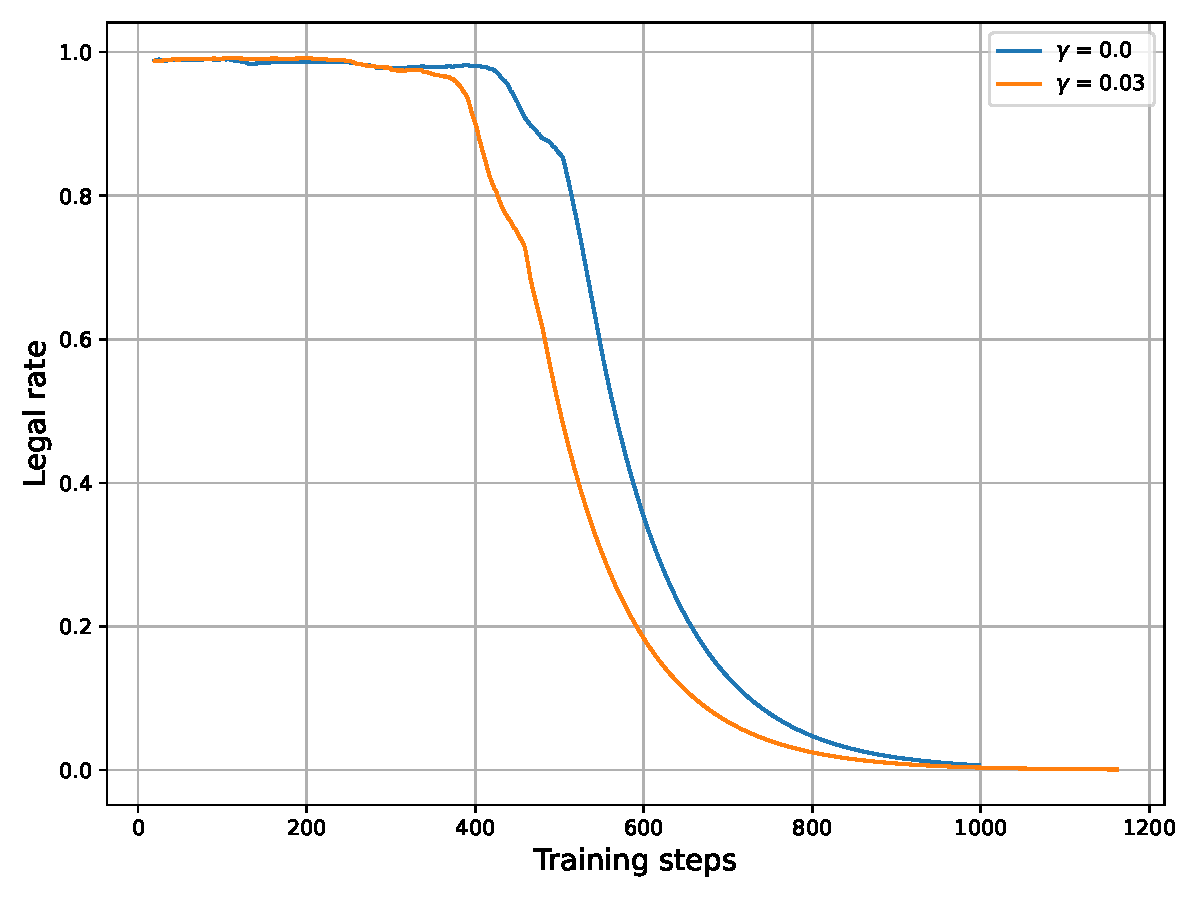
\includegraphics[width=0.49\textwidth]{sections/figures/rl_training_progress/overfit/ESPO/legal_rate.pdf}
    \hfill
    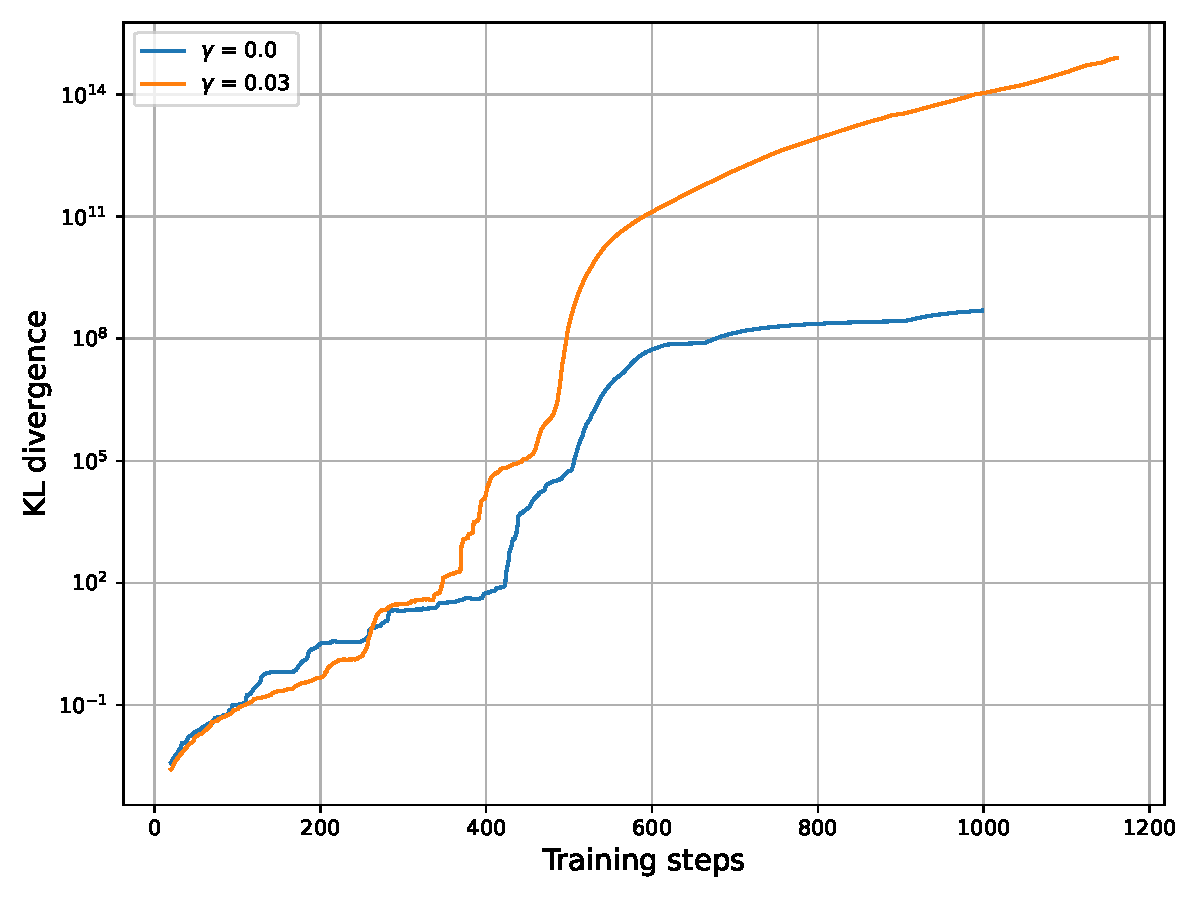
\includegraphics[width=0.49\textwidth]{sections/figures/rl_training_progress/overfit/ESPO/kl_divergence.pdf}
    \caption{The reinforcement learning training using ESPO with all diversity filtering mechanisms enabled. We observe that the model collapses and starts to generate illegal positions.}
    \label{fig:espo collapse}
\end{figure}





\section{Implementation details}
\label{sec:implementation details}

We provide an open-source implementation of the training algorithm we use at \url{https://github.com/naapeli/Generating-open-source-chess-puzzles}. All chess position evaluations were performed using the Stockfish engine \cite{stockfish}. To ensure reproducibility, we utilized a specific development build (dev-20260111-eb5a65ae), compiled on January 11, 2026, just before the release of Stockfish 18.
